% Sec. V, time evolution. Draft by Sohan, 22 Oct 2026. Drop-in replacement for section_5_time_evolution.tex.
%
% Data: the open-chain arm only. Every SNAP circuit was trained, compiled, realized and evaluated on the 100-site
% open chain (runs/<tag>/t<T>/chain/ladder.json and chain/newton/eval_*.json). No ring-trained circuit is used.
% The product-formula baseline is untrained and evaluated on the same chain (runs/<tag>/t<T>/baseline_o*.json).
% Snapshot of 22 Oct 2026, 01:20 PDT, frozen in data_snapshot/ (350 records); compiles are still running at
% t <= 4, t = 6 runs on Isaac's workstation, and only 2 of the 208 open-chain points have their fallback draws.
% Table I, the three data figures and every number in the text come from scripts/make_te_figures.py, which prints
% the text's numbers to te_text_numbers.txt. After `make_te_figures.py --refresh`, recheck the text against it.
% Rigorous baseline: snapevo-scratch/litbase/rigorous (Liu et al. bound). Liu orderings: litbase/mps_final.
% The old fig:synthesis (Sep data, catalysis era) is replaced by the main results figure, which keeps the label so
% the reference in the introduction still resolves. New bib keys Liu2026 and Caro2023 are in
% references_additions.bib. Technical details are in appendix_time_evolution.tex (app:te_details).
% Fig. te_circuit is still a placeholder.

\section{Time evolution}
\label{sec:time_evolution}

We now compile the time-evolution operator $e^{-iHt}$ of a spin chain. The procedure is the one of Sec.~\ref{sec:snap}. We fix a Clifford+$R_z$ circuit and an error $\epsilon(\vtheta)$, optimize the angles $\vtheta$, and then snap them onto the library one at a time, with the Hessian of $\epsilon$ deciding which snaps to try first. Two things change from state preparation. The target is a unitary, so the error has to be small for every input and not just for one state. The circuit is also translation invariant, so each angle is shared by many rotations and a single snap fixes all of them.

We compare every compiled circuit with product formulas that use the same gates, the same synthesis protocol and the same definition of the error. At an error of $10^{-3}$ per site, SNAP needs 3.3 to 3.4 times fewer T gates than the cheapest product formula when the chain is in a transverse field, and 1.3 to 2.1 times fewer without one, for times up to $t = 4$. Over every error the compiled circuits reach so far, the factor is 1.1 to 4.8 with the field and 1.1 to 3.9 without it. Product formulas whose number of steps is chosen from a rigorous error bound need 8 to 51 times more T gates than SNAP.

\subsection{Circuit and error}
\label{sec:time_evolution_setup}

We take the XXZ chain in a transverse field,
\begin{equation}
H = \sum_{i} \big( S^x_i S^x_{i+1} + S^y_i S^y_{i+1} + \Delta\, S^z_i S^z_{i+1} \big) + h_x \sum_{i} S^x_i ,
\label{eq:te_ham}
\end{equation}
with $S^{\alpha}_i = \sigma^{\alpha}_i/2$ and $\Delta = 0.25$, at two fields, $h_x = 1.6$ and $h_x = 0$. Times are $t = 1$, 2 and 4 in units of the inverse exchange coupling. Without the field a product formula needs no field layer, which makes $h_x = 0$ the easier case for the baselines of Sec.~\ref{sec:time_evolution_baselines}. \sg{Add $t = 6$ when Isaac's run comes back.}

The circuit is a brickwork of $D$ sublayers, shown in Fig.~\ref{fig:te_circuit}(a). Sublayer $\ell$ applies one two-qubit gate $G(\vtheta_\ell)$ to every bond of one parity, the even bonds when $\ell$ is even and the odd bonds when $\ell$ is odd. For $h_x = 1.6$ the gate is
\begin{equation}
G(\vtheta_\ell) = e^{-i(a\,XX + b\,YY + c\,ZZ)/2}\, \big[ R_x(e) \otimes R_x(f) \big]
\label{eq:te_gate}
\end{equation}
with $\vtheta_\ell = (a, b, c, e, f)$. For $h_x = 0$ we replace the single-qubit factor by $R_z(d) \otimes R_z(-d)$, so that $\vtheta_\ell = (a, b, c, d)$. We add this staggered rotation because the zero-field circuits train poorly at large depth without it. Each factor in Eq.~\eqref{eq:te_gate} is one $R_z$ rotation between Cliffords. For example, $e^{-icZZ/2} = \mathrm{CNOT}\,[I \otimes R_z(c)]\,\mathrm{CNOT}$, and the $XX$, $YY$ and $R_x$ factors follow from it by single-qubit Cliffords, as in Fig.~\ref{fig:te_circuit}(b). Every bond therefore carries five rotations, and a circuit of depth $D$ has $5D/2$ rotations per qubit.

All bonds of a sublayer share its angles. The circuit is then invariant under translation by two sites and is defined on any even number of sites, and it has only $5D$ bulk angles for $h_x = 1.6$ and $4D$ for $h_x = 0$, whatever the size of the system. The first-order product formula is one point of this family. Two sublayers with $a = b = \tau/2$, $c = \Delta\tau/2$ and $e = f = h_x\tau/2$ apply one Trotter step of length $\tau$.

The compiled circuit $U$ has to approximate $e^{-iHt}$ on every input. We test it on product states $|\phi_k\rangle$ whose single-qubit factors are drawn uniformly from the Bloch sphere. Such inputs are cheap to evolve with tensor networks, and a unitary learned from enough low-entanglement inputs generalizes to all inputs~\cite{Caro2023,Gibbs2025infinite}. For input $k$ the fidelity is $F_k = |\langle \phi_k | e^{iHt}\, U | \phi_k \rangle|^{2}$. With a fixed error per site, $F_k$ decays exponentially in the number of sites $N$, so we report the infidelity per site,
\begin{equation}
\epsilon = 1 - \frac{1}{K} \sum_{k=1}^{K} F_k^{1/N} ,
\label{eq:te_eps}
\end{equation}
averaged over $K$ inputs. This is the local infidelity of Ref.~\cite{Gibbs2025infinite} on a finite chain. Throughout this section $\epsilon$ means Eq.~\eqref{eq:te_eps} and $\epsilon_b$ is the budget on it. The fidelity of the whole chain is about $(1 - \epsilon)^{N}$, so $\epsilon = 10^{-4}$ on $N = 100$ sites leaves a fidelity of $0.99$.

We train, snap and evaluate on an open chain of $N = 100$ sites, with every state held as a matrix product state~\cite{Schollwock2011}. The training error uses $K = 12$ inputs. The $\epsilon$ we report uses $K = 8$ other inputs, so it is a held-out value. The references $e^{-iHt}|\phi_k\rangle$ come from a fourth-order product formula with a step small enough that its own error is negligible. We use an open chain rather than a ring because random product inputs build up entanglement linearly in $t$, and on a ring every bipartition cuts two bonds, which roughly squares the bond dimension. On the odd sublayers the two end sites have no partner, so each gets its own gate $R_z R_y R_z$ there, six angles per odd sublayer, trained together with the bulk angles. An end gate appears once per circuit, while each bulk gate appears $N/2$ times, so the end gates add at most 2.5\% to the T count. For every compiled circuit the held-out $\epsilon$ is between 0.92 and 1.05 times the training value, with a median ratio of $1.00$. \sg{This paragraph is the only part of the section that depends on the system-size question raised on 22 Oct. With an infinite chain, Eq.~\eqref{eq:te_eps} becomes the leading eigenvalue of the mixed transfer matrix~\cite{Gibbs2025infinite}, the end gates go away, and this paragraph shrinks to two sentences.}

\begin{figure}[t]
\centering
\fbox{\parbox[c][5.2cm][c]{0.93\columnwidth}{\centering\small
Placeholder for Fig.~\ref{fig:te_circuit}.\\[1ex]
(a) brickwork of $D$ sublayers on a chain, one gate $G(\vtheta_\ell)$ per bond,\\
end gates on the odd sublayers\\
(b) $G(\vtheta_\ell)$ as five $R_z$ rotations between Cliffords\\
(c) one stretch of a compiled circuit, rotations colored by T cost:\\
product formula with every rotation synthesized, against SNAP}}
\caption{The time-evolution circuit. (a) Each sublayer applies the gate $G(\vtheta_\ell)$ of Eq.~\eqref{eq:te_gate} to every bond of one parity, with the same angles on every bond, so the circuit is invariant under translation by two sites. On the odd sublayers each end site gets its own single-qubit gate. (b) The gate written as five $R_z$ rotations between Cliffords. The rotations by $a$, $b$ and $c$ act on the parity of the two qubits, and those by $e$ and $f$ on each qubit. (c) A stretch of the circuit at $h_x = 1.6$, $t = 4$ and $\epsilon = 10^{-3}$, with each rotation colored by its T cost, for the cheapest product formula (top) and for SNAP (bottom). \sg{Panel (c) follows David's suggestion on Slack (11 Oct), a colorbar for the T cost as in the tQPE paper.}}
\label{fig:te_circuit}
\end{figure}

\subsection{Optimizing the angles}
\label{sec:time_evolution_training}

For each field and time we train circuits of increasing depth. Each depth starts from three points: the first-order product formula of that depth, the optimum of the previous depth with identity sublayers appended, and the product formula with 0.1~rad of noise on its angles. From each start we minimize the training error by trust-region Newton steps. The Hessian comes from central differences of exact gradients, and each one serves several steps. A run stops when $\epsilon$ falls by less than a part in $10^{6}$ per step or reaches the truncation noise of the matrix product states, with no cap on the number of iterations. We keep the best of the three runs. Its error $\epsilon_0(D)$ is the floor of that depth, the error of the circuit before any angle is snapped. We stop adding depth once the floor falls by less than a factor of 1.5 over eight sublayers, or reaches $10^{-10}$. Figure~\ref{fig:te_floors} shows the floors. The depth needed for a given floor grows roughly linearly with $t$. This is the variational compression of Refs.~\cite{Lin2021compressed,McKeever2023classically,Gibbs2025deep,Gibbs2025infinite}, and it supplies the Clifford+$R_z$ circuit and the optimizer that SNAP assumes.

\begin{figure}[t]
\centering
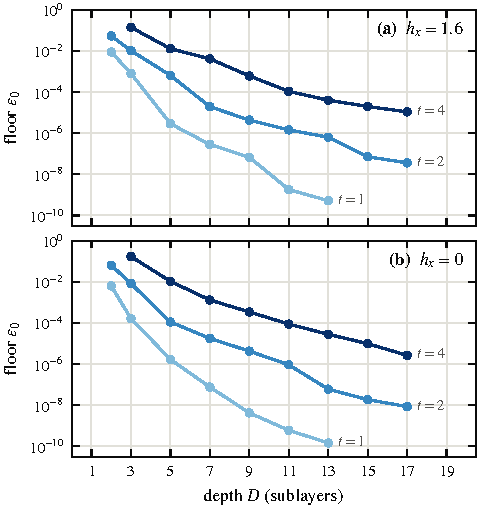
\includegraphics[width=\columnwidth]{fig_te_floors.pdf}
\caption{Floors of the trained circuits. The training error $\epsilon_0$ of the best circuit at each depth $D$, before any snap, on the 100-site chain, for $t = 1$, 2 and 4 (light to dark) at $h_x = 1.6$ (a) and $h_x = 0$ (b). \sg{The ladders at $t = 2$ and 4 are still being extended. Could move to the appendix if space is short.}}
\label{fig:te_floors}
\end{figure}

\begin{figure*}[t]
\centering
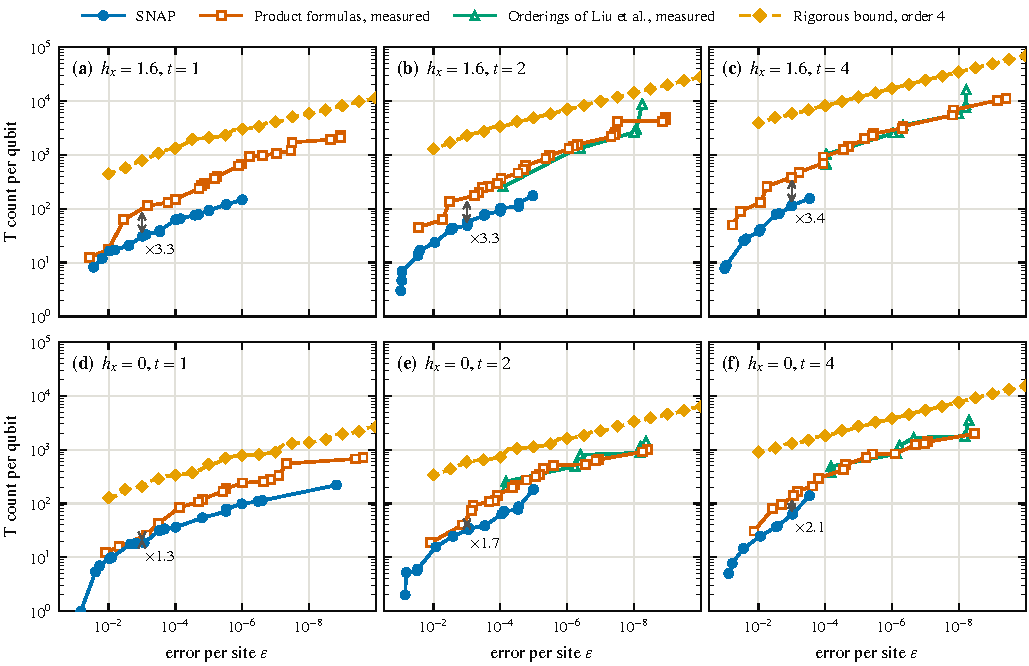
\includegraphics[width=\textwidth]{fig_te_tradeoff.pdf}
\caption{T count per qubit against the error per site $\epsilon$, Eq.~\eqref{eq:te_eps}, measured on 100 sites, with the error decreasing to the right. (a--c)~$h_x = 1.6$ and (d--f)~$h_x = 0$, at $t = 1$, 2 and 4. Circles are SNAP. Squares are the product formulas of order 1, 2 and 4 with measured error and the fallback branches drawn. Triangles are the orderings and field placements of Ref.~\cite{Liu2026} at orders 2, 4 and 6, measured on the success branch at $t = 2$ and 4. For our product formulas at these times, drawing the fallbacks raises $\epsilon$ by a median of 2\%. Diamonds are fourth-order product formulas with the number of steps and the synthesis precision chosen from the bound of Ref.~\cite{Liu2026}, plotted at their guaranteed $\epsilon$. Each series is its lower envelope, the cheapest circuit at or below each $\epsilon$. The arrows give the ratio of the product formula to SNAP at $\epsilon = 10^{-3}$, as in Table~\ref{tab:te_ratio}. \sg{SNAP points sit at their fallback bound until their draws run, Sec.~\ref{sec:time_evolution_snap}.}}
\label{fig:te_tradeoff}
\label{fig:synthesis}% the introduction cites fig:synthesis for the comparison with existing approaches
\end{figure*}

\subsection{Snapping shared angles}
\label{sec:time_evolution_snap}

The compiler is the loop of Sec.~\ref{sec:snap}, with three changes.

First, an angle of sublayer $\ell$ sets the rotation on every bond of that sublayer, $N/2$ bonds for even $\ell$ and $N/2 - 1$ for odd $\ell$. Snapping it to a library angle $\alpha$ costs $T(\alpha)$ per bond, about $T(\alpha)/2$ T gates per qubit. Every bulk angle has nearly the same multiplicity, so the loop still tries candidates in order of $T(\alpha)$. The end angles are re-optimized with the bulk after every snap. When the loop stops they are moved to Clifford or library angles where the budget allows, and the rest are synthesized (App.~\ref{app:te_details}).

Second, the error is no longer a sinusoid in each angle. An angle shared by $m$ rotations enters each overlap as a trigonometric polynomial of degree $m$, Eq.~\eqref{eq:shared_trig}. We fix that polynomial exactly from the overlap at equally spaced values of the angle, about 50 of them for most angles at $N = 100$, and it then gives the plug-in error at every library angle. We compute the Hessian of the training error over the free bulk and end angles from central differences of the exact gradient, Eq.~\eqref{eq:hess_fd}, and recompute it after every accepted snap. After each trial snap the free angles are re-optimized by the same trust-region Newton method used in training, again with no cap on the number of iterations.

Third, near the floor the loop has to leave room for the angles it does not snap. When $\epsilon_b$ is only a few times $\epsilon_0$, the loop could spend the whole budget on snaps and leave the remaining angles to be synthesized at a precision that costs more than the snaps saved. We therefore accept a snap only if the budget it leaves can still pay for synthesizing the rest, and we report the cheapest prefix of the accepted sequence, Eq.~\eqref{eq:prefix}.

We compile budgets in half decades from $\epsilon_b = 10^{-1}$ to $10^{-9}$, where the budget applies to the training error. Each budget is compiled at every trained depth whose floor is at most $\epsilon_b/1.5$, and the figures show the cheapest result at each error. \sg{Compiles at the tighter budgets are still running. So far the points reach $\epsilon \approx 10^{-6}$ at $t = 1$ with the field and $10^{-9}$ without it, $10^{-5}$ at $t = 2$ and $3 \times 10^{-4}$ at $t = 4$. Snapshot of 22 Oct, 01:20 PDT.}

When the loop stops, every rotation is one of three kinds. A rotation at a multiple of $\pi/4$ is exact and costs 0 or 1 T. A rotation at another library angle is exact on the success branch of its circuit and costs the expected T count of Eq.~\eqref{eq:rus}. A rotation that was never snapped is synthesized with the non-mixed fallback protocol of Ref.~\cite{Kliuchnikov2022}, at the precision that the remaining budget allows. We use no catalysis and no mixed synthesis anywhere in this section. A synthesized rotation takes its fallback branch with probability at most $0.1$, and we draw these branches at random in the $N = 100$ simulation, so the reported $\epsilon$ includes them. A library circuit whose failure cannot be undone exactly is corrected by a synthesized rotation of known precision, and we bound the effect of these corrections and add it to $\epsilon$ (App.~\ref{app:te_details}). \sg{The draws for the SNAP points have not run yet. Until they do, every SNAP point in the figures and Table~\ref{tab:te_ratio} sits at its fallback bound, which can only overstate its error. The bound moves $\epsilon$ by less than 1\% for 90\% of the points.}

\begin{figure}[t]
\centering
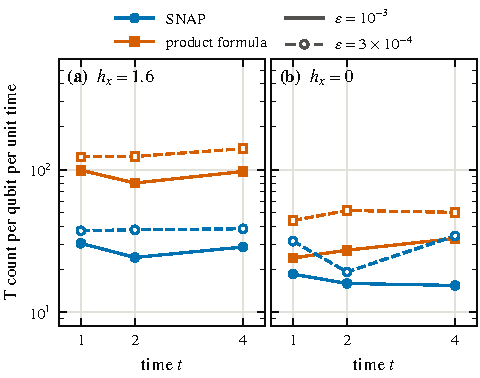
\includegraphics[width=\columnwidth]{fig_te_time.pdf}
\caption{T count per qubit per unit time against $t$ at fixed error per site, for SNAP (circles) and the cheapest measured product formula (squares), at $\epsilon = 10^{-3}$ (solid) and $3 \times 10^{-4}$ (dashed), for $h_x = 1.6$ (a) and $h_x = 0$ (b). Both are read off the lower envelopes of Fig.~\ref{fig:synthesis}.}
\label{fig:te_time}
\end{figure}

\subsection{Baselines}
\label{sec:time_evolution_baselines}

We compare against product formulas that use the same synthesis protocol, with their error obtained in two ways.

The first measures it. We split $H$ into the even bonds, the odd bonds and the field, and build formulas of order 1, 2 and 4~\cite{Suzuki1991} with $r$ steps. Every distinct angle is synthesized once at precision $\epsilon_{\mathrm{syn}}$ with the protocol of Ref.~\cite{Kliuchnikov2022}, and all its copies use the same circuit, so their synthesis errors add coherently. We scan the order, $r$ and $\epsilon_{\mathrm{syn}}$, measure $\epsilon$ for each formula exactly as for SNAP, on the same held-out inputs at $N = 100$ with the fallbacks drawn, and keep the cheapest formula at each error. This baseline relies on the same classical simulation as SNAP, and it is the strongest version of the conventional approach that we know how to build. The orderings and field placements of Liu \emph{et al.}~\cite{Liu2026} at orders 2, 4 and 6, measured on the same inputs, fall close to the same curve.

The second takes the error from a bound, as one would without a classical simulation. We use the ordering-aware Trotter bound of Ref.~\cite{Liu2026}, which is within a factor of 1.5 of the exact Trotter error for these formulas on 6 to 10 sites. We choose $r$ so that the bound, converted to a guarantee on Eq.~\eqref{eq:te_eps} at $N = 100$, meets the target, and we synthesize every rotation at an equal share of what remains. Fourth-order brickwork formulas are the cheapest at every time and error we tried. The error of this baseline is guaranteed rather than measured.

\sg{Isaac's third comparison, the trained circuit with every rotation synthesized and no snaps, has not been run. It separates the gain from compression from the gain from snapping. Sec.~\ref{sec:time_evolution_results} estimates it from rotation counts for now.}

\subsection{Results}
\label{sec:time_evolution_results}

Figure~\ref{fig:synthesis} shows the T count per qubit against $\epsilon$ at $t = 1$, 2 and 4. Table~\ref{tab:te_ratio} gives the ratio of the T count of the measured product formula to that of SNAP at three errors and every time. SNAP is cheaper than every product formula at every error reached so far. With the field the factor is 3.3 to 3.4 at $\epsilon = 10^{-3}$ for all three times and 1.1 to 4.8 over all errors. At $t = 1$, where the compiles reach furthest, it rises to 4.7 at $\epsilon = 10^{-6}$. Without the field the factor is 1.1 to 3.9, and largest at $t = 1$ near $\epsilon = 4 \times 10^{-8}$. At $\epsilon = 10^{-3}$ it grows with time, from 1.3 at $t = 1$ to 2.1 at $t = 4$. The gap is smallest at the loosest errors. At $t = 1$ it is a factor of 1.1 near $\epsilon = 10^{-2}$ with the field and near $2 \times 10^{-3}$ without it.

All of the saving comes from the cost of each rotation. Between $\epsilon = 10^{-2}$ and $10^{-5}$ a SNAP circuit spends 0.3 to 5.6 T gates per rotation, while the cheapest product formula spends 2.7 to 16. The trained circuits do not have fewer rotations. With the field they have 0.8 to 1.9 times as many as the cheapest product formula at the same error, and without it 1.2 to 6 times as many, because a zero-field product formula has three rotations per bond instead of five and needs few steps at these times. Compression alone, with every rotation synthesized as in the product formula, would therefore save little or nothing here. \sg{Replace the last sentence with the measured comparison once it is run.} The share of angles that end at Clifford angles falls with time and with the budget. At $\epsilon_b = 10^{-3}$ it is 64\%, 40\% and 10\% at $t = 1$, 2 and 4 with the field, and 71\%, 59\% and 41\% without it. Most of the rest end at library angles. None of the 174 circuits compiled at $\epsilon_b \geq 10^{-4}$ leaves an angle unsnapped. Below that, 10 of the 34 circuits do, up to 46\% of the angles in one of them.

The rigorous baseline is far more expensive. Between $\epsilon = 10^{-3}$ and $10^{-6}$ it needs 21 to 51 times more T gates than SNAP with the field and 8 to 21 times more without it. Most of this gap is the price of using a bound. The same formulas with measured error are already 3 to 15 times cheaper than with the bound. SNAP and the measured baseline both avoid that price because a classical simulation of the circuit is available, which is the setting this paper assumes.

% Generated by paper_draft/scripts/make_te_figures.py; do not edit by hand.
\begin{table}[t]
\caption{Ratio of the T count of the cheapest measured product formula to that of SNAP, at equal error per site $\epsilon$ on 100 sites, with the fallback branches of the product formulas drawn. SNAP points whose fallback branches are not drawn yet sit at their fallback bound, which can only overstate their error. A dash marks a time at which the compiled circuits do not yet reach that $\epsilon$.}
\label{tab:te_ratio}
\begin{ruledtabular}
\begin{tabular}{ccccccc}
 & \multicolumn{3}{c}{$h_x = 1.6$} & \multicolumn{3}{c}{$h_x = 0$} \\
$t$ & $10^{-2}$ & $10^{-3}$ & $10^{-4}$ & $10^{-2}$ & $10^{-3}$ & $10^{-4}$ \\
\hline
1 & 1.1 & 3.3 & 2.4 & 1.4 & 1.3 & 2.0 \\
2 & 2.4 & 3.3 & 3.9 & 1.4 & 1.7 & 2.5 \\
4 & 3.4 & 3.4 & -- & 1.7 & 2.1 & -- \\
\end{tabular}
\end{ruledtabular}
\end{table}
% generated by scripts/make_te_figures.py

\subsection{Cost per unit time}
\label{sec:time_evolution_perunit}

Figure~\ref{fig:te_time} shows the T count per qubit and per unit time. Up to $t = 4$ it changes little for SNAP. At $\epsilon = 10^{-3}$ SNAP spends 24 to 30 T gates per qubit per unit time with the field and 15 to 19 without it. The product formula needs 81 to 99 with the field, and without it rises from 24 at $t = 1$ to 33 at $t = 4$. At $\epsilon = 3 \times 10^{-4}$ SNAP spends 37 to 39 with the field, against 123 to 140 for the product formula. For the whole chain at $t = 4$ and $\epsilon = 3 \times 10^{-4}$, where the 100 sites keep a fidelity of $0.97$, SNAP needs $1.5 \times 10^{4}$ T gates and the product formula $5.6 \times 10^{4}$. \sg{$t = 6$ will show whether the gap opens with time.}

\subsection{Worst-case error}
\label{sec:time_evolution_opnorm}

The error per site is an average over inputs. A guarantee for every input needs the operator norm of $U - e^{-iHt}$, minimized over a global phase, which grows with $N$ and roughly with $\sqrt{\epsilon}$. \sg{Measure this relation on the open-chain circuits once the runs are done, and add the operator-norm version of Fig.~\ref{fig:synthesis} that Isaac asked for.}
